\chapter{Introducción}

El streaming (retransmisión) consiste en la distribución de contenido multimedia, de forma que el usuario consume dicho contenido a la vez que se descarga. Dentro de este campo encontramos el llamado live streaming cuya diferencia radica en que el contenido multimedia es retransmitido en directo, sin necesidad de ser grabado anteriormente por lo que el usuario lo consume en tiempo real.
En los últimos años estas tecnologías han experimentado un gran crecimiento y han surgido múltiples plataformas que lo soportan (youtube , twitch , periscope , bab) proporcionando a los desarrolladores distintas opciones para crear aplicaciones web que manejen estas tecnologías.
Por otro lado, otro mundo que ha crecido rápidamente en este tiempo es el mundo de los drones. Estos vehículos aéreos no tripulados, se pueden usar para la grabación o retransmisión de eventos incluyendo una cámara en su diseño.
Finalmente todos estos avances van de la mano del desarrollo de tecnologías web que permiten crear aplicaciones cada vez más sofisticadas y potentes aportando nuevas funcionalidades sin la necesidad de instalar nada en tu ordenador.
La temática principal de este proyecto gira entorno a todos estos campos, la recogida del contenido multimedia, procesado y su posterior retransmisión a través de una plataforma web que será YouTube.
A continuación se incluye una introducción al streaming y las tecnologías y protocolos que lo respaldan. También hablaremos de los drones y su relación con la distribución de contenido multimedia así como de distintas aplicaciones que permiten retransmisión en directo de eventos, principalmente YouTube que es el elegido para este proyecto.

\section{Streaming}

Como se ha mencionado anteriormente el streaming consiste en poder consumir contenido multimedia sin que este haya sido previamente descargado. Antes de la aparición de dicha tecnología en 1995 de la mano de la aplicación RealAudio, basada en la retransmisión de audio a través de internet, era necesario descargar y almacenar en el disco duro dicho contenido al completo antes de poder ser consumido.
Tras la aparición de esta primera aplicación de streaming de audio le siguieron otras muchas incluyendo además el vídeo, pero este progreso siempre ha ido ligado a un factor limitante, el ancho de banda que se encuentra estrechamente relacionado con la difusión de vídeo, ya que tanto como para retransmitir un evento como para consumirlo con cierta calidad y sin esperas necesitamos un ancho de banda aceptable, que en España con la llegada de la fibra óptica se ha conseguido en los últimos años. Otro factor que ha ralentizado el desarrollo, es el estado de los equipos ya que estos no poseían la suficiente potencia para visualizar correctamente estas transmisiones.
Otro de los campos en los que el streaming se está asentando es en el televisivo, plataformas como Netflix, HBO , Hulu o muchas otras están sustituyendo a la televisión tradicional. Estas plataformas permiten visualizar cierto contenido en cualquier momento sin estar sujeto a un horario, lo cuál es la principal ventaja de estas plataformas.
Con la expansión del streaming se desarrollo el live streaming, que consiste en retransmitir eventos en directo a través de internet. Con este fin se desarrollaron multitud de aplicaciones como YouTube live events, perispcope, yomvi … Que ofrecen la posibilidad de consumir o retransmitir evenos en directo.
A parte del entretenimiento, el streaming también es usado con otros fines como puede ser la enseñanza donde se obtiene una gran libertad ya que tanto alumno como profesor pueden estar en distintas partes del mundo. Uno de los ejemplos mas claros de este uso podemos observarlo en la medicina, donde se han hecho retransmisiones en directo de operaciones quirúrgicas de forma que tanto alumnos como otros profesionales de la medicina puedan aprender nuevas técnicas. Una de las areas donde se ha implantado esta tecnología es en la vídeo vigilancia, donde a través de la red IP se monitoriza la actividad del lugar deseado.


\begin{figure}[H]
    \centering
    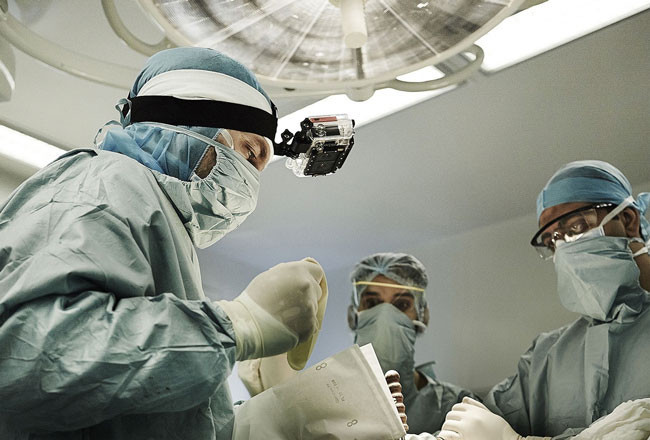
\includegraphics[width=100mm]{medicina.png}
    \caption{Streaming en un quirófano}
\end{figure}


A continuación se presenta un gráfico donde se puede ver como el consumo de contenido multimedia ha aumentado y la previsión del consumo en el futuro.

\begin{figure}[H]
    \centering
    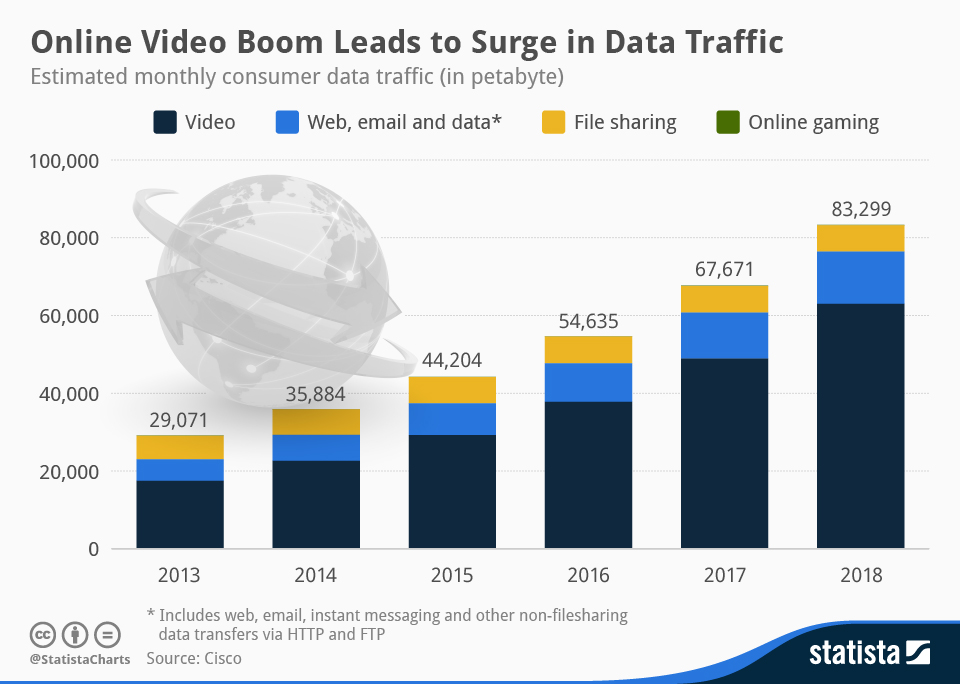
\includegraphics[width=100mm]{uso_datos_internet.png}
    \caption{Distribución tráfico de Internet}
\end{figure}

\subsection{Funcionamiento del Streamming}

Desde el punto de vista del usuario el uso del streaming es el siguiente. El usuario se conecta al servicio que le proporciona el contenido multimedia, dicho contenido se encuentra almacenado en servidores que contienen los archivos comprimidos en formatos conocidos como códec  MP3,VP8, AVI… Una vez establecida la conexión comienza la transmisión que está basada en protocolos “ágiles” de transporte como RTSP, RTCP, UDP etc... que serán explicados a continuación. La transmisión se hace en pequeñas partes de forma que se consigue una transmisión mas rápida al ser menos pesada. Por otro lado para poder garantizar una reproducción continua se incluye un buffer en el cual van siendo almacenadas partes del contenido, de forma que el usuario no necesita descargar el contenido completo del archivo sino que solo necesita pequeñas partes de él. 

En el proceso de streaming se deben tener en cuenta varios factores que pueden limitar la calidad del mismo. Desde el lado del consumidor el factor mas limitante es el ancho de banda, aunque con las nuevas velocidades de conexión casi cualquier compañía proporciona un ancho de banda suficiente. A continuación se adjunta las recomendaciones de ancho de banda de Netflix en función de la calidad de vídeo.

\begin{table}[H]
\centering
\begin{tabular}{|c|c|c|}
\hline
 CALIDAD & Mbps & GB POR HORA \\
\hline
STANDARD DEFINITION(SD) & 3 MB & 0,7 MB \\
\hline
HIGH DEFINITION(HD) & 5 MB & 3 MB \\
\hline
ULTRA HIGH DEFINITION(4K) & 25 MB & 7 GB \\
\hline
\end{tabular}
\caption{Ancho de banda remomendado en función de la calidad}
\end{table}

Si nos situamos en el lado emisor se deben tener en cuenta otros factores,

\begin{itemize}
    \item \textbf{Codec} , es un programa o dispositivo hardware capaz de codificar o decodificar una señal o flujo de datos digitales. El códec elegido afecta tanto en la calidad como en la velocidad de transmisión del archivo , ya que a mayor calidad de codificación mayor tasa de bits necesitamos.Uno de los mas usado es H264 para vídeo que esta dejando paso a su predecesor H265 ambos permiten codificar video de alta calidad.
    
    \item \textbf{BitRate}, el bitrate o tasa de bits representa la cantidad de bits que se envían por unidad de tiempo y es uno de los factores más importantes a la hora de producir una retransmisión de calidad aunque este factor está limitado por el ancho de banda de subida del que dispongamos. En este punto cabe destacar el uso del multi-bitrate que consiste en enviar distintas señales cada una con un bitrate diferente de forma que nos aseguramos que este contenido pueda ser consumido por todo tipo de conexiones. 
     
    \item \textbf{Key Frame}, también conocido como i-frame, este fotograma representa una imagen completa y sirve de referencia a las demás imágenes en la que el codificador solo almacena las diferencias entre una y otra. Cuanto mayor sea este valor menos datos se transmitirán pero peor será la calidad del vídeo. 
      
    \item \textbf{FrameRate},, son las imágenes por segundo con las que se reproduce el vídeo a mayor framerate mayor calidad y mas pesado será el archivo. 
    
\end{itemize}

\subsection{Protocolos Streaming}

Exiten diversos protocolos para sostener la tecnología streaming, en esta sección vamos a centrarnos en tres protocolos HLS, RTSP, RTMP y DASH  aunque para explicar dichos protocolos primero debemos hacer una breve introducción a RTP y UDP.
RTP son las siglas de Real-time Transport Protocol es un protocolo de nivel de sesión utilizado para la transmisión de información en tiempo real, como por ejemplo audio vídeo o datos. Junto a este protocolo se suele usar RTCP ( RTP Control Protocol )  es un protocolo de comunicación que proporciona información de control que está asociado con un flujo de datos para una aplicación multimedia. Este protocolo no transporta ningún dato por si mismo se encarga de transmitir paquetes de control, datos de la conexión, bytes enviados, control de calidad …
Estos protocolos se encapsulan sobre UDP (User Datagram Protocol) que a su vez constituye un protocolo de nivel de transporte que se encarga de enviar datagramas a través de la red sin necesidad de establecer una conexión previa, tampoco posee información de flujo ni confirmación por lo que los paquetes pueden llegar desordenados o no llegar, por este motivo se usa junto a RTCP que monitoriza y controla dichos paquetes.

\begin{itemize}
    
\item RTSP
    
Es un protocolo de transmisión en tiempo real (Real Time Streaming Protocol) establece y controla uno o muchos flujos sincronizados de datos, ya sean de audio o de vídeo. Es un protocolo no orientado a conexión, en lugar de esto el servidor mantiene una sesión asociada a un identificador, en la mayoría de los casos RTSP usa TCP para datos de control del reproductor y UDP para los datos de audio y vídeo. RTSP es similar a HTTP a excepción de que introduce nuevos métodos y necesita mantener el estado de la conexión. Los métodos mas importantes del protocolo son 

    \begin{itemize}
        \item \textbf{Describe},se solicita una descripción de un objeto multimedia contenido en el sevidor. Con esta petición se comienza el protocolo.
        \item \textbf{Setup}, especifica como serán transportados los datos que suele incluir el puerto para recibir los datos RTP (audio y video) y los datos de control RTCP.
        \item \textbf{Play},esta petición provoca que el servidor comience a enviar el flujo de datos.
        \item \textbf{Pause}, detiene temporalmente el flujo de datos.
        \item \textbf{Teardown}, finaliza el envió de datos y libera los recursos usados.
    \end{itemize}   

\item RTMP

Protocolo de mensajería en tiempo real, se trata de un protocolo basado en TCP que mantiene conexiones persistentes y comunicación en baja latencia. El flujo de datos es dividido en distintos fragmentos de forma que se entreguen flujos de información con la mayor cantidad de datos posible y sin problemas, este tamaño es negociado entre el cliente y el servidor. Por otro lado RTMP define varios canales para el intercambio de datos, estos canales pueden estar activo simultáneamente. Este encapsula por encima suya en MP3 o AAC el audio y en FLV el video. 
Este protocolo presenta distintas variaciones puede usarse con conexiones TLS/SSL (RTMPS) junto con encriptación (RTMPE) , encapsulado dentro de HTTP (RTMPT) o sobre UDP (RTMFP).


\item DASH

Dynamic Adaptative Streamming Over HTTP también conocido como MPEG-DASH que es un protocolo de streaming adaptativo cuyo objetivo es modular la tasa de bits en función del estado de la red. Para ello su idea principal es disponer del contenido en diferentes calidades y fragmentado de forma que cada segmento temporal puede ser enviado en distintas calidades. DASH usa HTTP como su protocolo de transporte lo que simplifica las conexiones a la hora de atravesar NAT’S o firewalls.

\begin{figure}[H]
    \centering
    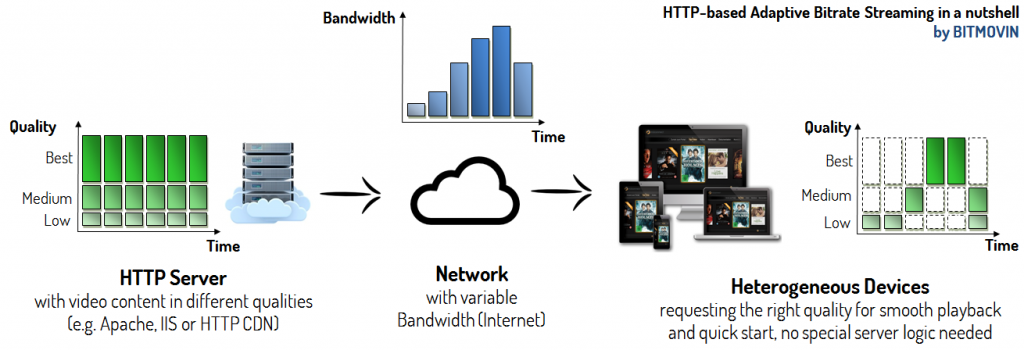
\includegraphics[width=150mm]{dash.png}
    \caption{Arquitectura DASH}
\end{figure}

\item HLS

HTTP Live Streaming es un protocolo basado en HTTP implementado por Apple. Divide el flujo en pequeñas partes que son transmitidas, dando lugar al cliente a elegir el tipo de transmisión que mas se adapte a su conexión. También implementa un mecanismo de codificación basado en AES.

La arquitectura del protocolo se divide en un servidor que se encarga de codificar y encapsular la entrada de vídeo para ello utiliza H.264 como códec de vídeo y MP3, HE-AAC o AC-3 como códec de audio. Un distribuidor que se trata de un servidor web convencional que procesa las peticiones y devuelve los recursos pedidos y por último un cliente que recibe el flujo de vídeo.

\begin{figure}[H]
    \centering
    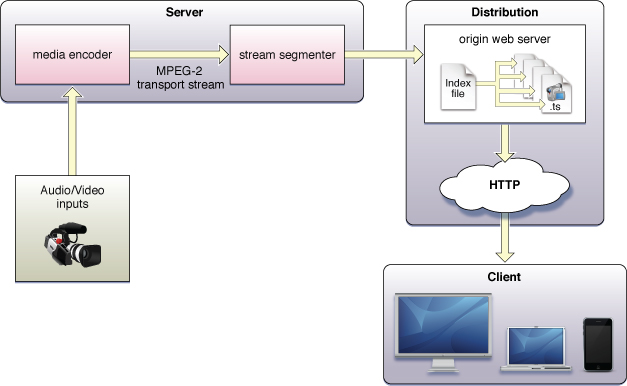
\includegraphics[width=150mm]{HSL.png}
    \caption{Arquitectura HLS}
\end{figure}    
\end{itemize}

\section{Youtube}

Desde su creación en 2005 YouTube ha experimentado un crecimiento brutal, de forma que hoy en día cuenta con más de mil millones de usuarios a nivel mundial subiéndose alrededor de 300 horas de vídeo por minuto.
Tras su lanzamiento solo un año después, en 2006 , google compró la compañía por 1.650 millones de dólares, tras esto se aumentó el número de vídeos que la plataforma contenía a lo que le siguieron multitud de avances , se incluyeron listas de reproducción y vídeos relacionados , traducción a distintos tipos de idiomas en forma de subtítulos, canales en los cuales cada usuario puede publicar su contenido para que sea visto , se dio la posibilidad de añadir anuncios a los vídeos , vídeos de mayor duración , desarrollo de una aplicación móvil, contenido de alta definición y eventos en directo.
Pero no todo es positivo, uno de los problemas mas importantes que YouTube arrastra es la piratería y la publicación de contenido inapropiado. Debido a la gran cantidad de volumen de vídeos que maneja YouTube se hace muy complicado controlarlo todo de forma que la piratería esta proliferando en esta plataforma, se puede encontrar música o películas publicadas sin posesión de los derechos de autor, para intentar paliarlo YouTube creo el Content-Id de forma que los propietarios de los derechos de autor puedan identificar y gestionar fácilmente su contenido en YouTube. Aún así se acusa a Google de hacer la vista gorda ante este tipo de contenido.

\subsection{YouTube Live}

A principios del año 2011 YouTube puso a disposición de los usuarios la posibilidad de emitir eventos en directo de forma gratuita. Para la realización de estos eventos es necesario unicamente un codificador que recoja el flujo de datos de tu ordenador y lo transfiera a YouTube, en este momento existen bastantes alternativas tanto gratuitas como de pago. Estos eventos pueden ser programados para una fecha concreta, poseen opciones de privacidad, puede emitir más de un evento a la vez y pueden ser estos grabados. 
Actualmente YouTube esta perfeccionando otra modalidad de emisión en la cual la retransmisión se realiza inmediatamente, a diferencia de los eventos el proceso de transcodificación es llevado a cabo por YouTube quien automáticamente detecta la resolución y frecuencia de tu transmisión.
Otra de las funcionalidades que YouTube está incorporando actualmente es la retransmisión en directo con calidad 4K y de grabaciones de 360º.

Todos estos avances han supuesto un gran salto ya que cualquier usuario sin una gran infraestructura puede realizar una emisión en directo, a continuación se adjunta una tabla con los requisitos mínimos de las emisiones.


\begin{table}[H]
\centering
\begin{tabular}{|c|c c|}
\hline
 CALIDAD & RESOLUCIÓN & TASA DE BITS \\
\hline
240P & 426X240 & 300-700 Kbps \\
\hline
480P & 854X480 & 500-2000 Kbps \\
\hline
720P & 1280X720P & 1500-4000 Kbps \\
\hline
1080P & 1920X1080 & 3000-6000 Kbps \\
\hline
4k/2160P a 30 FPS & 3480X2160 & 13.000-34.000 Kbps  \\
\hline
\end{tabular}
\caption{Ancho de banda recomendado en función de la calidad}
\end{table}

\section{Vehículos Aereos no tripulados}

UAV (Unmanned Aerial Vehicle), coloquialmente conocidos como drones. Se trata de un vehículo volador controlado de forma remota. Los drones se encuentran formados por un material ligero para evitar sobrepeso pero resistente, motores y hélices que son los encargados de mantener al UAV en el aire, baterías que aporten la energía necesaria para su funcionamiento y  el control de vuelo donde se encuentra el cerebro del aparto dentro de él podemos encontrar sensores, memorias, microprocesadores o actuadores, todo ello acompañado de un software que ayude al control remoto del mismo. A estos componentes básicos pueden añadirse extras como por ejemplo GPS o una cámara.

\begin{figure}[H]
    \centering
    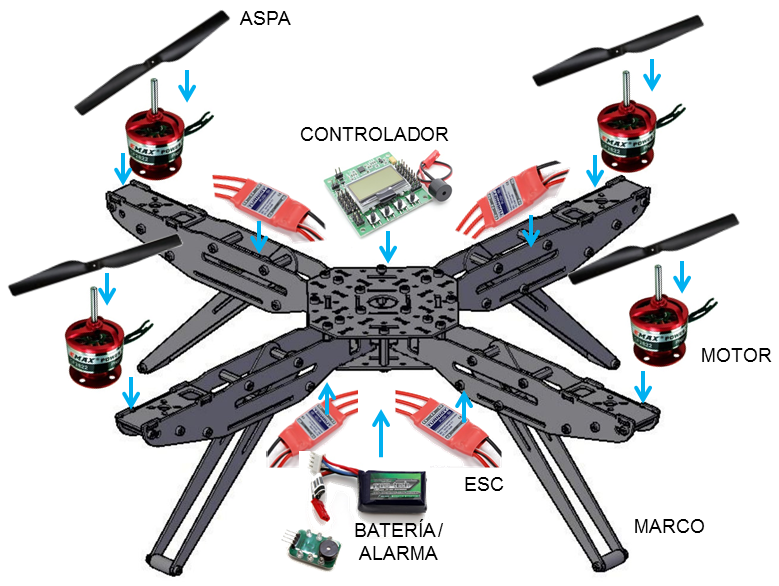
\includegraphics[width=100mm]{partesdronebasico.png}
    \caption{Partes UAV}
\end{figure}

Dentro de los UAV podemos encontrarnos con dos grandes tipos. Por un lado nos encontramos con los UAV de uso militar conocidos como UCAV (Ummaned Combat Air Vehicle), diseñado para su empleo militar, generalmente van armados. Estos aviones carecen de piloto humano a bordo. Las misiones de los drones se realizan generalmente bajo el control humano en tiempo real. Por otra parte están los UAV de uso civil que son los más habituales estos pueden desarrollar distintos tipos de tareas y muy variadas a continuación se listan algunas de ellas

\begin{itemize}
    \item Realización de trabajos que los humanos no quieren desempeñar, como puede ser control y manipulación de sustancias nocivas o explosivas.
    \item Entrega de paquetes, este campo aún está en fase de pruebas pero Amazon entre otras compañías están perfeccionando este método para un futuro no muy lejano.
    \item Retransmisión eventos, cine, fotografía, incorporando una cámara al UAV podemos obtener distintos planos con relativa facilidad por ejemplo el usado en el mundial de Brasil 2014 para captar todos los detalles del acontecimiento.
    \item Tareas de salvamento marítimo, se han desarrollado UAV los cuales son capaces de transporta salvavidas hasta el lugar del accidente de forma que las víctimas pueden usarlos hasta que llegue el socorrista.
    \item Juegos, también es usado en el campo del ocio, por ejemplo actualmente existen carreras de drones.
    \item Agricultura, usados en la agricultura de precisión, donde proporcionan análisis de datos en tiempo real volando sobre los terrenos velozmente y consiguiendo datos estadísticos por medio de los sensores a bordo. Con estos datos se produce una cartografía específica con información importante para su gestión de forma que se mejora la productividad

\end{itemize}

\begin{figure}[H]
    \centering
    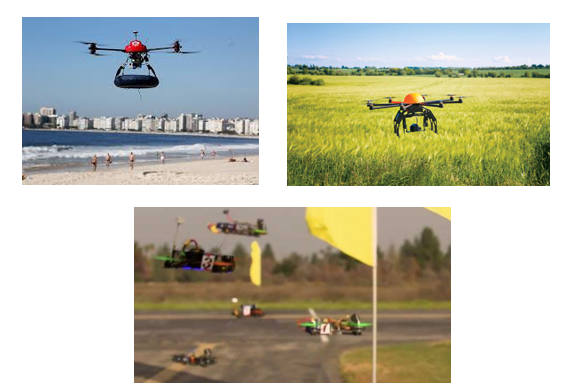
\includegraphics[width=100mm]{UAV.png}
    \caption{Distintas Partes UAV}
\end{figure}

Por último cabe destacar que estos aparatos podrían ser usados para fines delictivos, por ejemplo podrían ser usados para realizar un ataque terrorista, otro de las preocupaciones se centra en la privacidad ya que pueden ser usados para vulnerar la privacidad de las personas, por otro lado también preocupa la congestión del tráfico aéreo ya que a día de hoy no están preparados para evitar colisiones  y se debe llevar acabo un nuevo desarrollo del control de tráfico aéreo. Con estos aparatos también se puede contribuir a la retransmisión ilegal de eventos como podría ser un partido de fútbol o un concierto. La legislación presenta bastantes vacíos legales en lo que al vuelo de UAV se refiere.

\section{Antecedentes}

Como apoyo a este proyecto, sobre todo en el ámbito del manejo de UAV, tenemos trabajos anteriores realizados por alumnos de la URJC, todos ellos apoyados en la plataforma JdeRobot que nos proporciona herramientas para el manejo y control de estos dispositivos.

\subsection{JdeRobot}

JdeRobot es una plataforma de desarrollo de software para aplicaciones de robótica y visión por ordenador donde se incluyen sensores, actuadores y software inteligente. JdeRobot proporciona un entorno basado en componentes distribuidos comunicándose entre si mediante ICE.  También proporciona herramientas y librerías que proporcionan vistas y capacidad de teleoperación entre otras funcionalidades.

\subsection{Tecnologías web en JdeRobot}

Este trabajo fin de grado realizado por Aitor Mártinez consiste en una plataforma web que consta de cuatro clientes Camera ViewJS, RGBD ViewerJS,  KobukiViewerJS  y  UavViewerJS. Estas herramientas se comunican directamente con los servidores de JdeRobot sin necesidad de intermediarios, dicha comunicación se realiza a través  de WebSockets. Para familiarizarnos un poco más con el proyecto se explicaran brevemente las cuatro funcionalidades de la plataforma

\begin{itemize}
    \item Camera ViewJS, este cliente nos permite visualizar las imágenes tomadas por una cámara conectada al dron.
    \item RGBD ViewerJS, proporciona los datos de color y profundidad
    \item Kobuki ViewerJS, se trata de un teleoperador capaz de manejar y monitorizar datos de los robots Kobuki y Pioneer del laboratorio de la URJC.
    \item UAViewerJS, a través de esta herramienta es posible tele operar drones a la vez que se pueden visualizar los sensores del dron.
\end{itemize}

\begin{figure}[H]
    \centering
    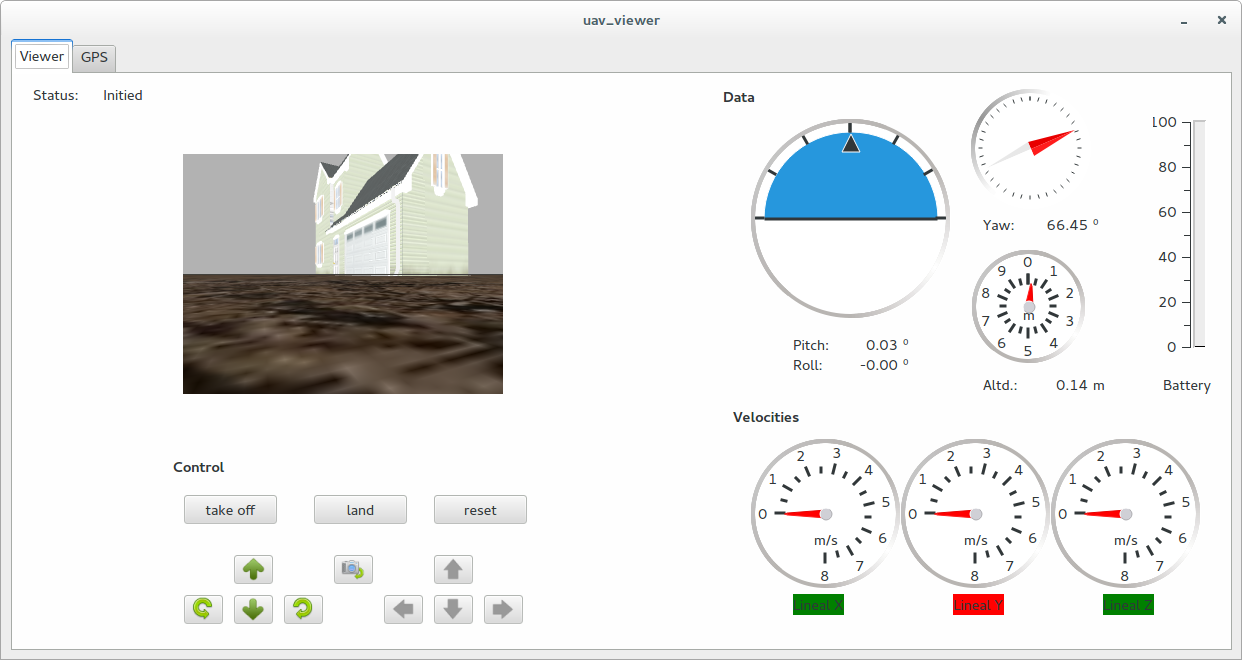
\includegraphics[width=100mm]{uav_viewer.png}
    \caption{Interfaz UAViewerJS}
\end{figure}

\subsection{Drone WebRTC}

Este proyecto fue realizado por Iván Rodríguez y consiste en combinar la tecnología WebRTC, con las herramientas proporcionadas por JdeRobot de forma que el resultado final es una aplicación web en la que podemos tele operar un cuadricoptero con la ayuda de controles y de un flujo de vídeo capturado por una cámara incorporada en el dron.

\begin{figure}[H]
    \centering
    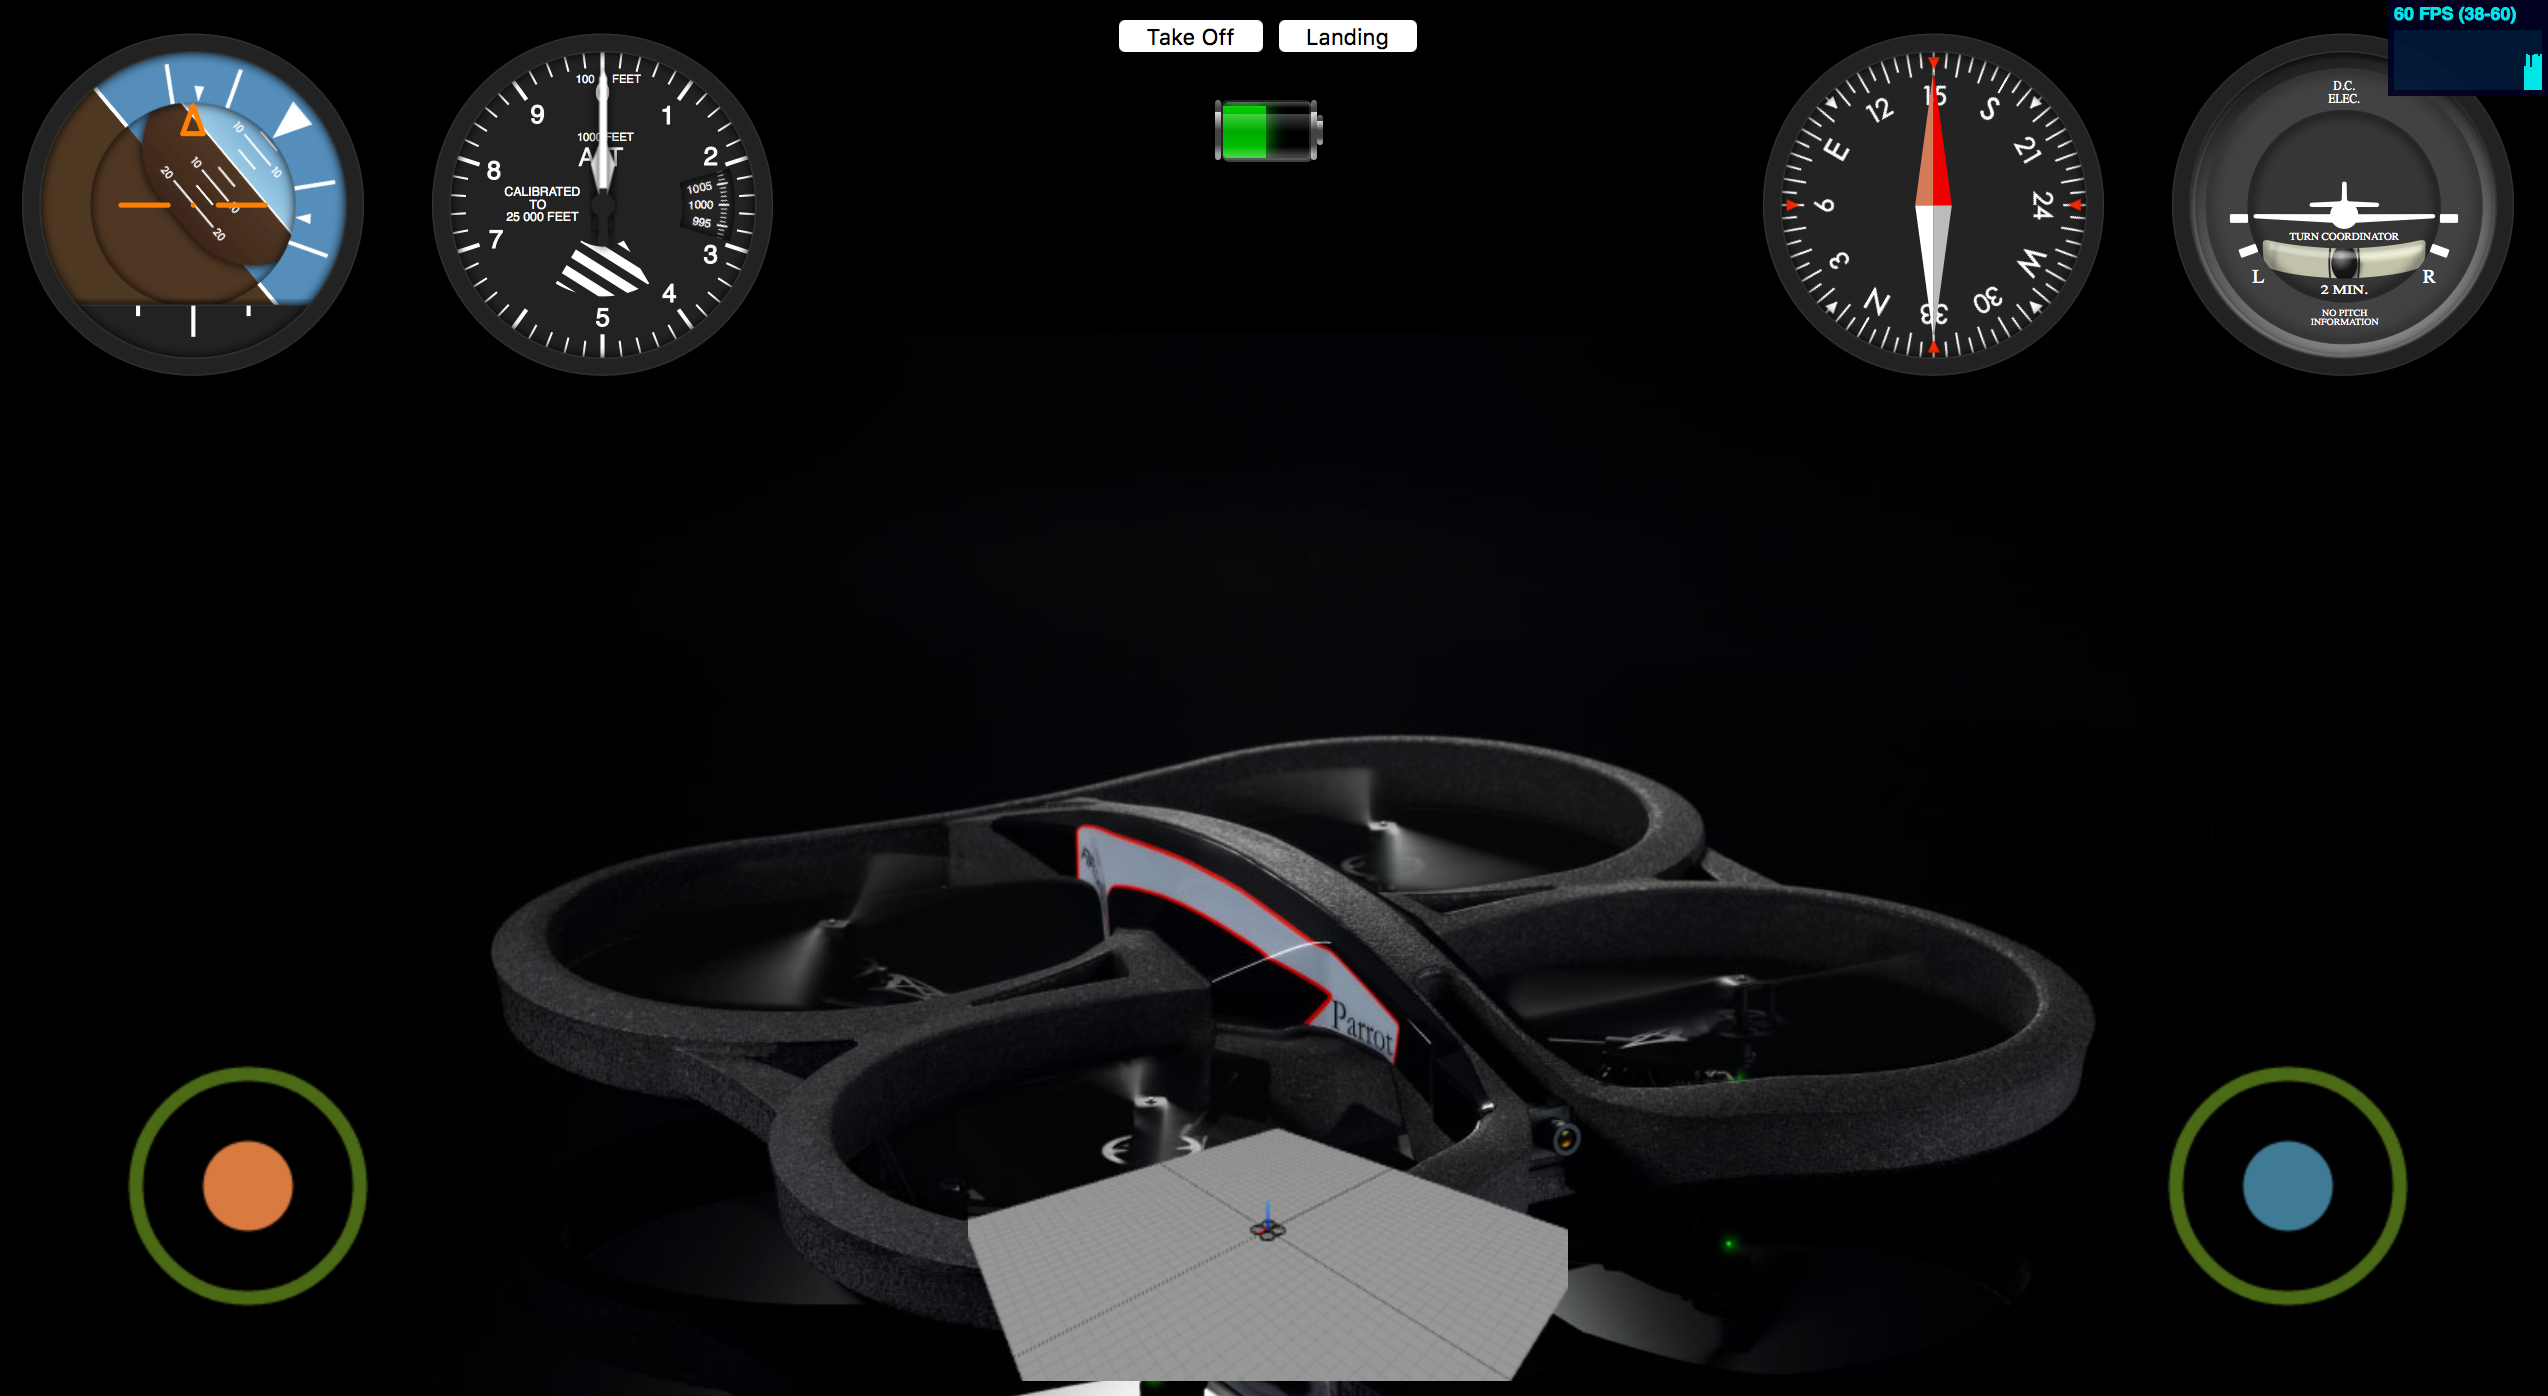
\includegraphics[width=100mm]{droneRTC.png}
    \caption{Interfaz de manejo Dron Remoto}
\end{figure}

Para la comunicación entre el dron y el ordenador local se usa la herramienta UAViewer, mencionada anteriormente. Desde un ordenador remoto se dan las instrucciones al dron y se controlan sus sensores, estas instrucciones son enviadas al ordenador que se comunica con el dron a través de WebRTC en tiempo real sin necesidad de servidores intermedios.

\begin{figure}[H]
    \centering
    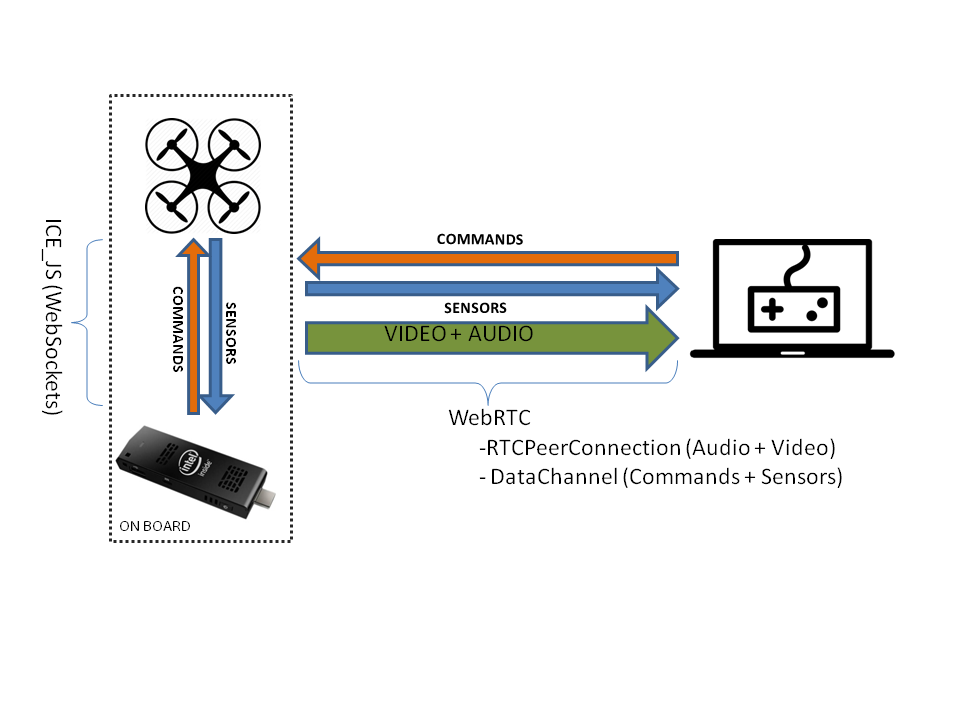
\includegraphics[width=130mm]{arqDroneRTC.png}
    \caption{Arquitectura de la aplicación}
\end{figure}

En el proyecto que se presentara a continuación se hace uso de las herramientas proporcionadas por JdeRobot y YouTube, con el objetivo de crear aplicaciones que recojan un flujo audivisual y sea publicado en YouTube a tiempo real.

Una vez puesto en contexto el proyecto a continuación se presentaran los objetivos del mismo así como las tecnologías usadas y la explicación del software desarrollo para dar paso finalmente a las conclusiones.
